\section{Development workflow}
\label{sec:github}

To manage and host the code of the web application, Konnektid's developers use Github. It is an application built on top of Git, a distributed version control system popular for its branching and merging functionalities~\cite{git}. As Git is originally based on command line, Github provides a clearer interface to visualize all Git events such as commits, merges, and more. 

Konnetid uses private repositories to store code, which are similar to public repositories except that they are not accessible to everyone: users need permission from the repository's owner if they want to see and modify its content.

\subsection{Environments}
\label{ssec:env}

Konnektid's website is deployed in three distinct environments, defined by the code itself but also by their own configuration for the application. The workflow is described on {\sc figure}~\ref{fig:githubFlow}.

\begin{figure}[h]
    \centering
    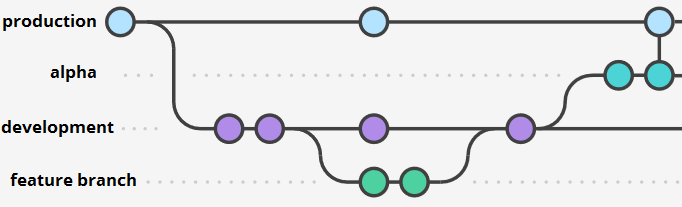
\includegraphics[scale=0.9]{figure/githubFlow.png}
    \caption{A diagram representing the Github workflow.}
    \label{fig:githubFlow}
\end{figure}

\textbf{development} is a directory for tasks currently being worked on, each of them in a local branch called \guillemotleft{} feature branch \guillemotright{}. Feature branches should be short lived, ideally not more than a few days, otherwise they cause integration issues because of the tasks other developers finish in the meantime. When the code is ready, the branch is merged in \textit{alpha}. 

\textbf{alpha} is a pre-release of new features, useful to provide further tests, fix remaining bugs, and make sure that everything is compatible with \textit{production}. The rest of the Konnektid team also has access to it, so that they can see and try out the latest functionalities, and eventually suggest some last changes to be made (for instance in the copywriting). Once everything is approved and fully tested, the code is released in \textit{production}.

\textbf{production} contains the code actually published on \url{https://www.konnektid.com/}.

When implementing an important modification in the code (for instance, change the general navigation), a \guillemotleft{} feature flag \guillemotright{} is used. It is a boolean, defined in the configuration files, that decides whether or not the new feature should be displayed in the branch. This technique assures that the critical changes will not affect the other branches.

A piece of code does not automatically move from \textit{development} to \textit{production}. First, it has to pass a certain number of tests before being committed and pushed. Then, it is manually reviewed: this is clarified in {\sc subsection}~\ref{ssec:reviewing}.

\subsection{Reviewing process}
\label{ssec:reviewing}

When a piece of code is ready to be merged, first in \textit{alpha}, the developer who implemented it opens a pull request~\footnote{User-friendly interface for notifying others of the completed feature and discussing proposed changes.} for it, with a \guillemotleft{} state/need review \guillemotright{} tag. Then, another member of the development team will take a look at the changes. This verification has three main goals:

\begin{itemize}[noitemsep]
	\item Verify that the changes fulfill their goal;
 	\item Check the quality of the code (for instance the indentation);
	\item Make sure that the merge will not cause any conflicts.
\end{itemize}

If something is wrong, the reviewer replaces the previous tag by a new one, \guillemotleft{} state/need improvement \guillemotright{} with a comment in the pull request to describe what needs to be enhanced. This allows the reviewee to efficiently iterate on it. Otherwise, if everything is fine, the reviewer adds a \guillemotleft{} state/approved \guillemotright{} tag and merges the branch in \textit{alpha}.

This process is rather efficient but very time-consuming, and not completely reliable as humans can make mistakes. To reduce this risk, Konnektid is introducing continuous integration (\guillemotleft{} CI \guillemotright{}) with Jenkins, an open source automation server~\cite{jenkins}. 

CI is a practice based on frequently integrating local code into the shared repository, where it is verified by an automatic build. It is meant to reduce integration issues, and if there are any it helps detecting them earlier. At the moment, CI in Konnektid is very basic and only performs a few tests on \textit{alpha}, but the goal is to improve it step by step in order to achieve continuous integration, continuous delivery (\guillemotleft{} CD \guillemotright{}) and fully automated testing. CD aims at safely releasing changes in \textit{production} as soon as a pull request is merged, so that it is faster to get feedback from the users and therefore easier to update.

Github is a very efficient communication tool for developers, and it really facilitates team work and code sharing. However, there are also non-developers in the Konnektid team, who do not use Github but still work on the same goals and projects. {\sc section}~\ref{sec:management} explains how this is managed, and how communication is handled.